\documentclass[pra,amssymb,showpacs,showkeys]{revtex4}
%\documentclass[pra,showpacs,showkeys,amsfonts]{revtex4}
\usepackage[T1]{fontenc}
\usepackage{textcomp}
\usepackage{graphicx}
%\documentstyle[amsfonts]{article}
\RequirePackage{times}
%\RequirePackage{courier}
\RequirePackage{mathptm}
%\renewcommand{\baselinestretch}{1.3}
%\RequirePackage[german]{babel}
%\selectlanguage{german}
%\RequirePackage[isolatin]{inputenc}
\usepackage[usenames]{color}
\newcommand{\Red}{\color{Red}}  %(VERY-Approx.PANTONE-RED)
\newcommand{\Green}{\color{Green}}  %(VERY-Approx.PANTONE-GREEN)


\def\ddarrow{{\swarrow\mkern-18mu\nearrow}}
\def\cddarrow{{\searrow\mkern-18mu\nwarrow}}
%
% Small help for images
\def\reserve#1#2#3{\setbox0\hbox{}\wd0=#1
                   \ht0=#2\special{#3}\box0}
\begin{document}



\title{Aesthetics and scarcity\\
       A physics perspective on ornament\footnote{Presented at the
{\em Data Ecology Workshop Part II} at the Time's Up laboratories - Linz/Austria 12th - 14th May. URL http://www.timesup.org/laboratory/DataEcologies/index2005.html}}

\author{Karl Svozil}
\email{svozil@tuwien.ac.at}
\homepage{http://tph.tuwien.ac.at/~svozil}
\affiliation{Institut f\"ur Theoretische Physik, University of Technology Vienna,
Wiedner Hauptstra\ss e 8-10/136, A-1040 Vienna, Austria}


\begin{abstract}
Human aesthetics is developed as a function of decryption.
Decryption is analyzed in terms of computation,
thus providing some principles
by which artists may design appealing virtual reality environments.
While too condensed coding makes a decryption
of a work of art impossible and is perceived as chaotic by the untrained mind,
too regular structures are
perceived as monotonous, too orderly and not very stimulating.
It is also argued that, due to human
predisposition, aesthetics is inevitably based on natural forms.
\end{abstract}

\pacs{89.20.-a,89.75.-k,01.70.+w}
\keywords{Interdisciplinary applications of physics, complex systems, philosophy of science}
\maketitle

\begin{quote}
\begin{flushright}
{\footnotesize
dedicated to Hans Frank d. J\"ungeren\\
painter, teacher and friend}
\end{flushright}
\end{quote}


\section{Simple questions}

Suppose you are in New York City, in midtown Manhattan, and you have ten minutes to spare. Where would you rather be: on Park Avenue? or in Central Park?  Don't think about it - what is your first reaction?

Park Avenue offers modernity; it is dominated by artistic structures created by valiant human imagination.
Central Park offers an artificial ``natural'' habitat,
created by valiant human landscape gardening.
Shouldn't all the trees and plants of Central
Park appear boring compared to the magnificence of Park Avenue's skyscrapers?

Nonetheless, I suspect that many or perhaps even most people would prefer Central Park over Park Avenue for just idling around. (I am not considering here the curiosity of suburbanites studying man-made canyons.) Why have so many people left the city centres in favour of rural surroundings?  Why is hiking and vacationing in beautiful natural habitats a means to refresh our minds?

One could also ask where one would choose to live if one were in a galaxy far, far away, shaken by Star Wars: on the planet Naboo? or on Coruscant?  Again, I suppose most people would choose the natural beauty of Naboo (at least after the siege of the Trade Federation is lifted).

Virtual realities - digitally created landscapes and habitats - may someday offer a chance to spend a holiday inside a totally artificial environment created by the digital artist.  At the present time, I suspect that most of us would dislike spending an entire holiday in one of the current generation of virtual reality installations, and would in fact rather undergo the rigors of travel in order to visit uncontrolled, natural spots far away.  Would it not be much more risk-free, convenient, personalised, funny, satisfactory and also cheaper to go virtual?  The artist, then, will want to provide surroundings that people will find most pleasing, or else fail to attract customers and audience.

There may be a simple explanation for the human preference for the natural.
This explanation runs against many modern artistic philosophies, such as International Style architecture,
``modern art'' paintings and modern ``classical'' music,
which upon constant exposure may be either monotonous and dull,
or irritatingly irregular and erratic, to the majority of people.
For the artist, the advantage of these styles is that they are systematic
and may be implemented with relative ease.
The aesthetics I suggest, by contrast, may impose a high burden on those who create virtual human habitats.


\section{An aesthetics of nature-beauty}


We propose that to a large degree aesthetics are derived from natural forms,
both ontogenetically and phylogenically.
The human experience of art, at least where beauty and appreciative
psychological responses are concerned, is informed by
the variations of natural forms such as clouds, rocks,
leaves, waves, or the songs of birds.
(Two such structures are depicted in
Figs.~\ref{2005-ae-foliage}\&\ref{2005-ae-China_MountEverest_MER_FR_Orbit09148_20031130_hires}.)
All human creations, in particular hermetic virtual realities,
must cope with this human predisposition, which limits the
plasticity and adaptability of human perception.
Regardless of the artistic motive, neglect of this
condition may result in a sense of provocation and
ugliness for the person experiencing the creation.
\begin{figure}
%\centerline{\reserve{19.0cm}{19.0cm}{pdf: image width 19.0cm (2005-ae-foliage.jpg)}}
\centerline{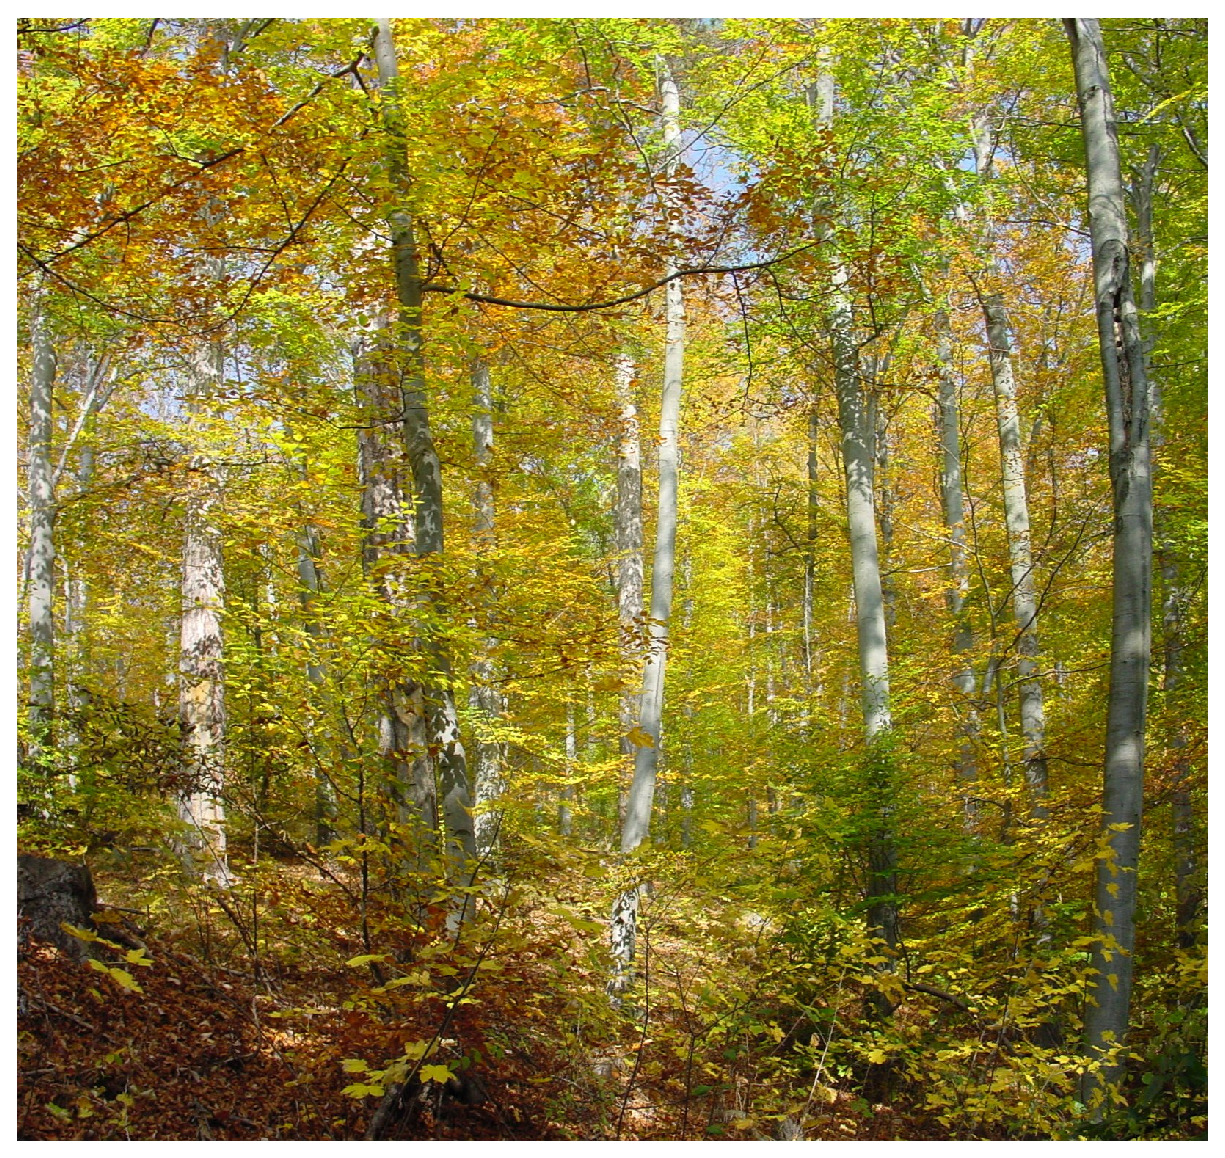
\includegraphics[width=19cm]{2005-ae-foliage}}
  \caption{Autumn foliage near Baden, Lower Austria, Oct. 15, 2000
(\copyright Karl Svozil)}
   \label{2005-ae-foliage}
 \end{figure}
\begin{figure}
%\centerline{\reserve{19.0cm}{19.0cm}{pdf: image width 19.0cm (2005-ae-China_MountEverest_MER_FR_Orbit09148_20031130_hires_s.jpg)}}
\centerline{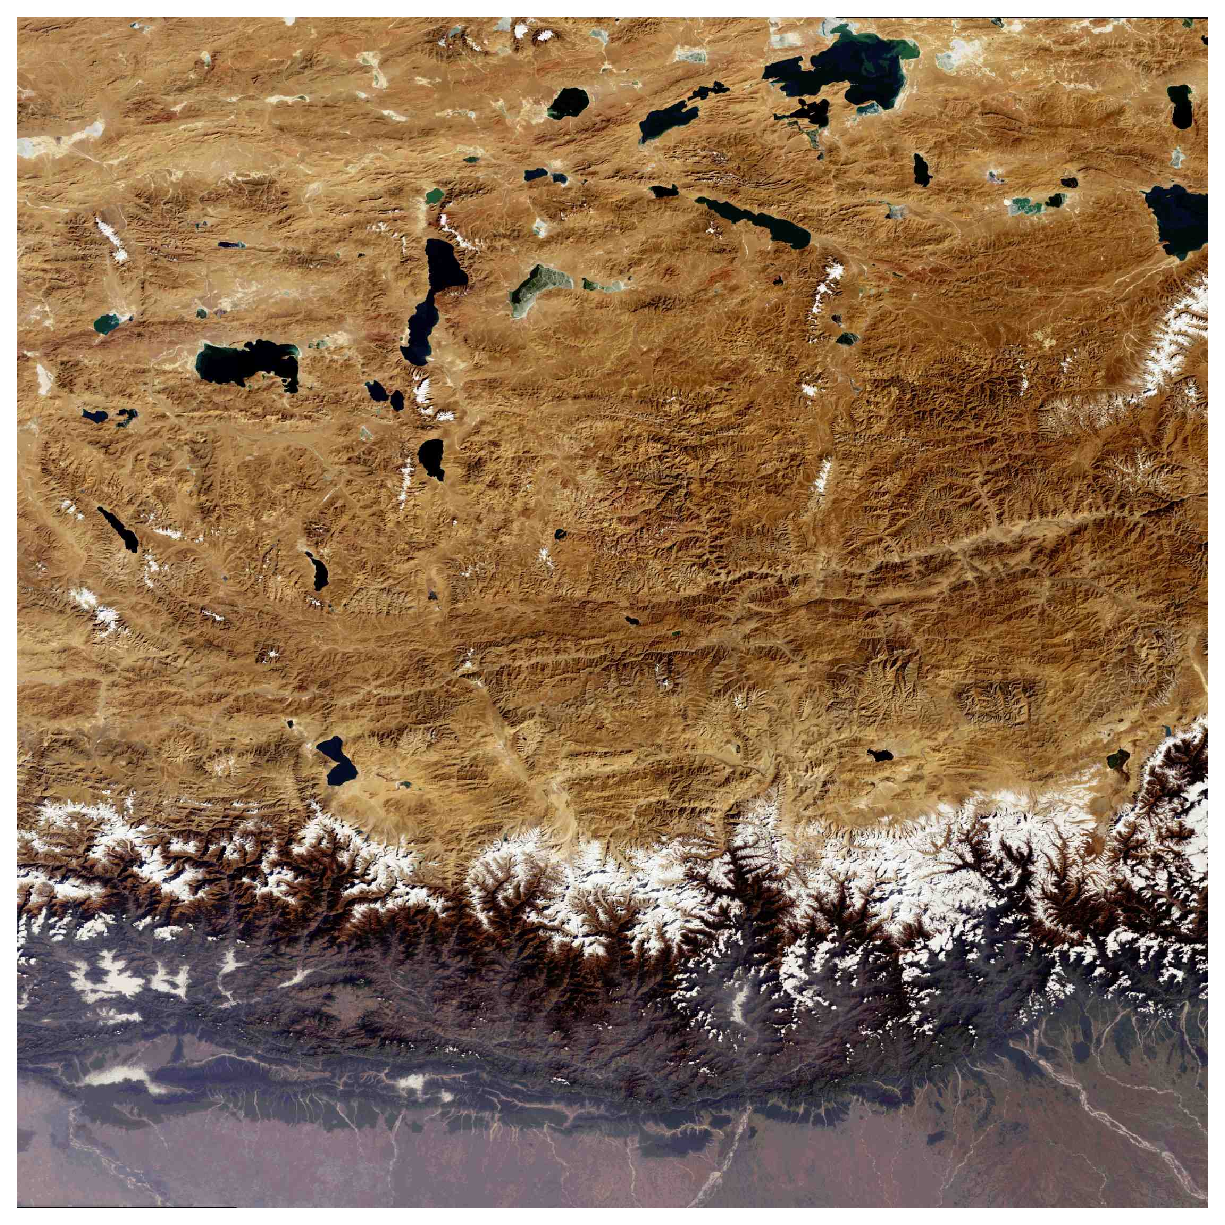
\includegraphics[width=19cm]{2005-ae-China_MountEverest_MER_FR_Orbit09148_20031130_hires_s}}
   \caption{Mount Everest as seen by MERIS at orbit \# 09148 on Nov. 30th, 2003
(\copyright ESA/MERIS)}
   \label{2005-ae-China_MountEverest_MER_FR_Orbit09148_20031130_hires}
 \end{figure}


One issue in the creation of virtual realities---and
also in contemporary architecture and the arts in general---is
the avoidance of monotony and uniformity,
despite the scarcity of available algorithmic,
imaginative or monetary resources \footnote{
In particular, architecture suffers from austerities
of form and lack of sophistication, which are sometimes externally
imposed upon the architects by financiers and engineers,
and which are sometimes self-inflicted in the name of style.
Conversely, music and some graphical arts have taken an
entirely opposite turn towards an aggregation of complexity
and the increase of information density per time or
space---in its extreme form promoting incomprehensible, irritating noise.}.
In this paper,
we will propose an aesthetics built upon what will be called ``nature-beauty��
(in German ``das Natursch�ne��
\footnote{
Compare Hegel's concept of ``das Natursch{\"o}ne'' (``beauty of nature'') \cite{bense}
which is contrasted to  ``das Kunstsch{\"o}ne'' (``beauty of art''),
although Hegel used a top-down system based on the human mind and
its superior artistic expression
instead of the bottom-up approach proposed here.}).
We will speak of ``natural entities,''
by which we mean specifically traditional forms occurring
in the natural human habitats of the past or in the rural settings of the present
\footnote{
We do not have in mind every form occurring in nature.
For example, a concrete wall is also a natural form by an extended definition;
but we do not include it in our considerations,
since we do not want to surrender to unbounded arbitrariness.}.


One assumption of nature beauty is the heuristic \textit{law of decryption}: every pattern and law
will eventually be decrypted, and the decryption process is central to the
human aesthetic experience. The more complex a pattern in terms of
description and production, the more difficult is its decryption. For the
person embedded in an aesthetic environment, if the decryption comes too
fast and easy the result will be boredom; conversely, if the decryption is
too difficult, the result will be perplexity and irritation.

\textit{Descriptional complexity} can be characterised by the algorithmic information content
\cite{chaitin2,chaitin3,calude:02};
i.e., by the length of the shortest program able to generate that pattern or form.
\textit{Computational complexity} \cite{calude1,bennett-utm,bennett1}
is a measure for the amount of time and
memory (space) required to generate the pattern or form from the algorithm.
For example, a very short subroutine of only a few lines can generate a very
large pattern or form, but it may take a very large amount of time and
memory to accomplish this. The resulting pattern, then, is descriptionally
simple, but computationally complex.

A related principle is the heuristic \textit{law of aesthetic complexity}. At one extreme, plain structures
appear monotonous; at the other extreme, totally stochastic structures
appear irritating. That is to say, where patterns are simple and easily
recognised, the person experiencing them quickly loses interest; and equally
true, where there is no recognisable pattern at all, the person will also
lose interest in the apparent randomness.

Art takes place in the region between monotony and irritation,
between order and chaos.
Of course,
the mere absence of monotony and randomness is no sufficient criterion for
art, but it can be safely stated that it is a necessary one. Any attempt to
push the artistic boundaries either towards monotony or towards
stochasticity must consider the human mind, which might not be sufficiently
plastic to cope with the results.

Consider, for instance, the extremes of white noise and brown noise. White
noise is a type of noise that is produced by combining with equal weight all
different frequencies together.
White noise is thus characterised by a constant frequency spectrum $1/f^0$ and is too stochastic
and random to be perceived as music; it is extremely irritating to most
human ears. Some compositions by Gy\"{o}rgy Ligeti or John Cage may serve as
examples, where a great deal of randomness is intentionally introduced as a
matter of style---a style that many people find irritating and
incomprehensible. At the other extreme, we have brown noise---which takes
its name from Brownian motion, the apparently random bouncing of
molecules---exhibiting step-wise ``random walk'' behaviour with a frequency
spectrum $1/f^2$.
Brown noise appears monotonous and boring.

At the mid-point between these extremes of noise, we find what we might term
``pure music,'' which can be characterised by a frequency spectrum of about $1/f$. This type of
``noise'' may be termed ``fractal'' or self-similar ``noise''
\cite{voss-75,voss-78,gard-78,taylor-99}.


The term ``noise,'' of course, was coined to describe sound, but the
statistical analysis is easily applied to any mode of perception involving
pattern recognition. For examples of ``noise'' in graphic or visual art, we
may look to modernist paintings. ``White noise'' in paintings would, of
course, consist of a canvas painted over with an even, uniform coat of grey
paint (and there are some examples in modern art which very nearly approach
this ideal). ``Brown noise'' would be random shapes or splotches in random
colours at random locations on the canvas (and, again, there are some
modernist paintings which very nearly answer to this description). ``Fractal
noise'' in painting would consist of the regular and rigid application of
self-similar patterns, along the lines of the well-known images produced by
the Mandelbrot set. Such images are common in some computer graphics. What
is the effect on the viewer of these types of ``noise'' when exhibited in
paintings? Many viewers find all of these varieties of drawings to be
incomprehensibly dull, which is to say lacking in any aesthetic quality at
all
\footnote{
To be fair, these forms have their adherents, and I take the
relative popularity of these creations to be an indication of the utter
ignorance and obtuseness of audiences, who suspend their own standards and
judgements, deferring to fashionable opinions. The poet Handke has
exemplified such tendencies to the extreme in his play
``Publikumsbeschimpfung'' (Engl. translation ``audience bashing''), which
confronts the benevolent and over-tolerant audience with absurd slander and
insults. The author had the questionable privilege to see these principles
at work after he and his friend (presently a renown Viennese academic
himself) re-enacted the ``Publikumsbeschimpfung'' in front of a university
audience of learned scholars and students plus company, which truly seemed
to enjoyed the piece which obviously intended to insult them; and even sat
through the reading of three full pages of the Viennese phone book.---They
did not give up; we gave up!}.

``Noise'' is descriptionally simple, even if computationally complex. Very
few lines of code are required to produce an even and uniform whiteness; or
a random scattering of shapes; or an endless fractal pattern. For the
artist, descriptional simplicity (``very few lines of code'') means that he
or she has relatively little thinking to do to produce the ``art.'' By
contrast, nature-beauty imposes heavy algorithmic costs on the creators of
virtual realities and arts in general, requiring a structural richness that
exceeds the power of contemporary computers by orders of magnitude.

To illustrate, let us consider how Nature herself creates nature-beauty. In
terms of algorithmic information content, it takes about 4 million
nucleotides (the basic molecules forming the nucleic acids DNA and RNA), and
about 4 thousand genes, to describe the simple bacterium Escherichia coli
(E. coli). This is the genome of E. coli, which for present purposes we may
equate with lines of code and functional segments of code.
Humans have about 1,000 times more nucleotides
than E. coli (around 3 billion), and an estimated 40,000 to 60,000 genes.
Every cellular entity on earth can be assumed to lie within those bounds.
The phenotype---that is the bodily creature --generated from these codes is
quite beyond the capability of contemporary computers. Even ``mere'' protein
folding remains one of the most difficult computational challenges of our
time. This compares indirectly to the exorbitant computational resources
needed to simulate an entire city in detail within a virtual reality.

Ultimately, the above theses will have to be corroborated or falsified by
experience and neurophysiological modelling. They relate, in some respects,
to Chomsky's system of transformational grammar. One of the possible tests
would be to differentiate between the ontogenetic and the phylogenetic parts
of the thesis. Children who grow up in rural surroundings might, for
instance, show very similar aesthetic preferences when compared to urban
children, although their environmental experiences vary widely. The same
should be true for people from very different environmental, cultural,
social and ethnic backgrounds.

\section{Garden gnome virtual architecture?}
\label{subsec:mylabel1}

Several arguments can be brought forward against an aesthetics build upon
nature-beauty; some will be discussed below.


\subsection{Kitsch: ridiculing nature-beauty}

A clever demonstration directed against the aesthetics of
nature-beauty has  been devised by Udo Wid, a Viennese artist
and physicist. He planted a garden gnome into
a flower pot, such that only a very tiny upper part of its red cap was
visible. The gnome was surrounded by plants. Many people were actually taken
in by this arrangement. This instalment seemed to prove the
absurdity of any claims of the existence of nature-beauty---after all, an
aesthetics being blinded by a planted garden gnome cannot possibly have any
value.

However, I take Udo Wid's example not as evidence against the theory of
nature-beauty, but as just another indication of how easily people can be
seduced to perceive beauty while really being confronted with kitsch or even
trash. One might even ask: so what?

\subsection{Ugliness as a by-product of progress}


One artistic task is to expand upon existing forms, and sometimes such
expansion results in provocation and even ugliness. We might ask whether
provocation and ugliness are the inevitable companions of aesthetic
expansion.

I think not. Occasionally, provocation may accompany creativity, but it is
not a necessary element of artistic quality. Some groups of ``artists'' have
made it to their primary business to provoke, so that the provocation itself
is seen as sufficient justification for the art
\footnote{
In my opinion,
this has less to do with art than the need to attract attention. With
sufficient publicity, artists may create a market for their work; with
sufficient success, they may achieve an intellectual hegemony that
effectively excludes dissidents from monetary and academic resources.}.

Creativity that results in ugliness cannot properly be called progress, no
matter how intellectually and spiritually challenging. While the initial
provocation may prove stimulating and produce some expansion in the artistic
palette, the perpetuation of ugliness on ever larger scales is not a
promising programme
\footnote{
Here again, some would plead for an aesthetics
of unbounded relativism, asserting that ugliness is a subjective experience.
My answer to them is rather simple: I do not think so! Having stated this, I
acknowledge that the perfection of ugliness might be a stimulating
challenge, although not from an aesthetic point of view. Perhaps some
Foundation for Relativism in Art might endow a challenge prize for the
designer who is able to create the ugliest and most offensive virtual
universe possible.}.




\subsection{Artistic dominance}

Academically established schools of artistic taste have been able to
dominate contemporary arts and architecture to a large degree. However, the
most successful and popular artistic creations of our time do not follow
such conformist trends. For instance, when the writer and director George
Lucas and his team created dwellings for the Star Wars Episodes I and II,
they deliberately chose Renaissance-style palaces for the residence of the
Queen of Naboo. Even for Coruscant, seat of government for the Galactic
Republic and the Empire that supplanted it, they invented an architecture
not resembling any Bauhaus or other academic style. Indeed, perhaps the most
striking and effective cinematic use of the Bauhaus and International styles
was in connection with the terrors of Fritz Lang's \textit{Metropolis}. I would suggest that
these styles are effective for a tale of horror precisely because they make
people uncomfortable
\footnote{ Let me state a harsh and personal reply to
those artists and engineers who disguise  an aesthetics which is
based on natural forms: be advised that most of your customers prefer
natural habitats over simplified synthetic ones. You may like it or not, but
those customers will vote with their feet and their wallets against your
shallow perception of modernity. You may be fairly successful in print; you
may win prizes and be selected in tenders by committees of peers; you may
even be allowed or encouraged to build some similar creations for which the
20th century has become so (in)famous: the structureless skyscrapers, the
buildings made with pre-cast concrete slabs, and the bunkers. But you will
not achieve the thing that matters most, which is a virtual habitat in which
people silently hang around and pretentionless enjoy their living.}.

Most of this critique is not entirely new
\cite{wolfe-86,charles-89,krier-98}, and neither is the attempt to recover beauty
through natural forms. What may be new is the idea that the limits of
aesthetics may be due to the human condition, a heritage of how we perceive
the world, and the bounds imposed by algorithmic information and complexity.

\subsection{Scarcity of resources}

One of the most influential critiques of nature-beauty was formulated in
1908 by Alfred Loos in his pamphlet ``Ornament und Verbrechen'' (English
translation ``Ornament and Crime'')  \cite{loos}:
ornamentation
is expensive; and resources diverted to decoration are wasted with regard to
the functional value of the decorated objects. Those resources could for
instance be much better invested for leisure or for an increase in
productivity. Loos' principle can be pointedly stated by the following
question: why build one pretty house with ornamentation when you can have
two ugly ones for the same price?

Such thoughts blended in well with Frederick Winslow Taylor's ``The
Principles of Scientific Management''
\cite{taylor-1911}  written in 1911
%http://www.netmba.com/mgmt/scientific/
in the USA, as
well as the social fantasies of the Bolsheviks in the USSR. While such
principles improved productivity and had a substantial impact on the growth
of the economic output, they also increased the monotony of work and the human environment in general.
Certain
qualifications and benefits of craftsmen such as variety, identity,
significance and autonomy were abandoned. Charlie Chaplin's ``Modern Times''
is a persiflage of these circumstances. The products became cheap,
affordable and disposable but at the same time monotonous, insignificant,
dull and without charm.
We should ask ourselves to what extent
this tradeoff between charm and abundance has been justified.

To give an example: for the functionalist, a street lamp is just a street
lamp emitting light; nothing else. No matter how ugly the lamp looks, as
long as it serves its purpose by emitting light. If the total cost of
ownership is low, all is well in functional terms. What Loos and other
modernists did not recognise was that any street lamp has an indispensable
added value: by daylight, it is perceived by everybody not according to its
function as a street lamp, but as a kind of street furniture or decoration.
At day, the functional value of light emission is insignificant; what
matters instead is the design itself.

The same applies to the decoration of facades. Ornamentation of buildings
increases the cost of production and the efforts that go into it without
immediate functional value to the tenants; however, it serves another,
equally valuable purpose to a much greater audience: it appears pretty and
beautiful. An avenue or a court framed by buildings which are ornamented
looks less monotonous and austere than the same avenue or court with plain
facades. Without ornamentation, objects of everyday life appear cheap and
ugly.

One immediate reaction of customers is not to buy such things, to throw them
away immediately, or at least to get rid of them as soon as possible. This
may be one of the reasons why American products often sold better than the
same products from the former Soviet block. In Eastern Europe, nobody
attempted to imprint added values, because almost by Soviet definition, the
product needed to serve only its intended functional value.
Prettiness became equated with bourgeois decadence
\footnote{
On the contrary, consider the ``repressance''-type architecture of the Stalin time,
such as the main building of Lebedev University.}.
And as scarcity
dominated, any incentive to buy and enjoy consumption was discouraged. Let
me mention an anecdote: during an extended visit to Moscow in 1986, I
attended a performance of the Bolshoi theatre in the Kremlin. The audience
virtually cried out at a ball scene---they were so desperate for beauty and
ornament! This is different from surplus societies and supply-sided
markets---at least for those who can afford---where added value is an
important marketing factor.

A mere programmatic commitment to ornamentation does not solve the problem
of its cost, though. After all, Loos did not criticise ornamentation per se,
but the extra cost associated with it, which is not met by any immediately
recognisable functional value. Loos even suggested using naturally
ornamented panels and templates such as wood or stone as a substitute for
expensive human-crafted ornamentation.

Alas, natural ornamentation materials such as stones and wood are also expensive
and not affordable by everyone
(compare recent laminate floorings carrying photo reproductions of wood).
And as can be seen
from the beautiful parquet flooring recovered recently in the Palais
Liechtenstein, Vienna, depicted in Fig.~\ref{2005-ae-flooring},
even laying natural panels
requires high craftsmanship and geometric sophistication.
\begin{figure}
%\centerline{\reserve{19.0cm}{24.5cm}{pdf: image width 19.0cm (2005-ae-parkett.jpg)}}
\centerline{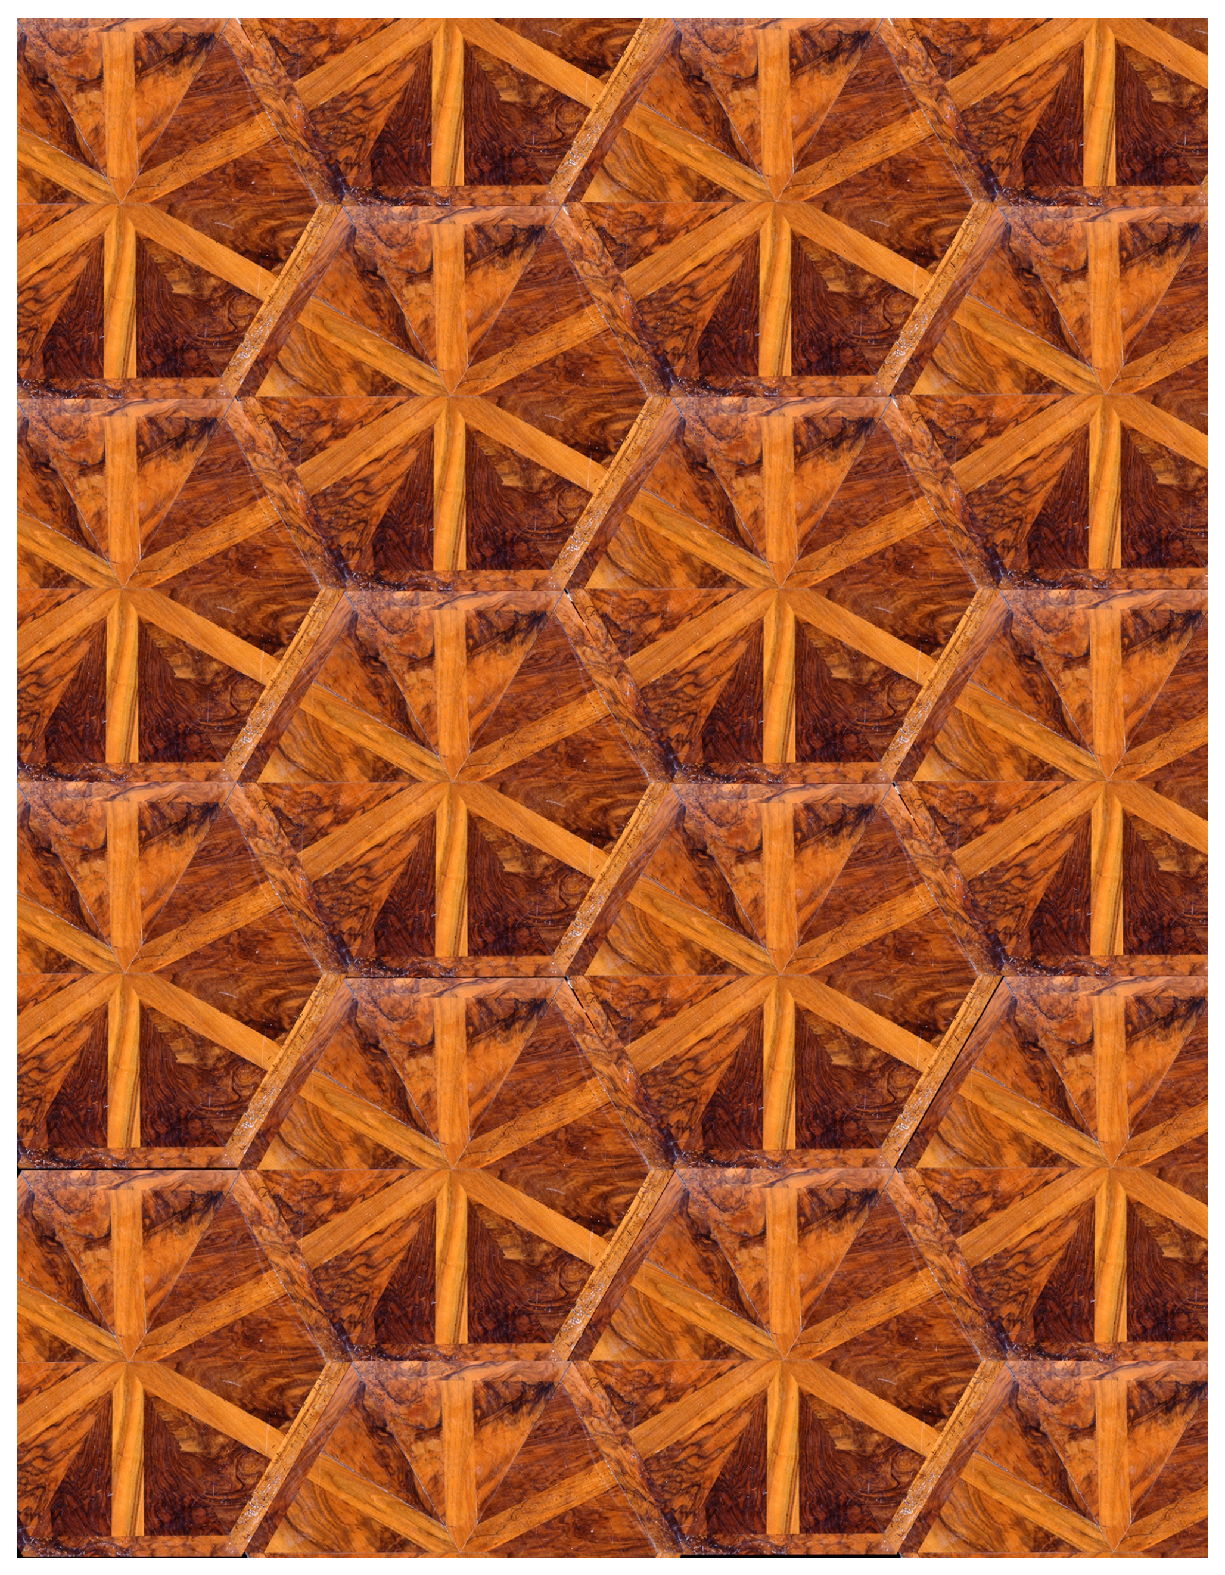
\includegraphics[width=19cm]{2005-ae-parkett}}
   \caption{Parquet flooring  in the galery rooms of the Garden Palais
 Liechtenstein, late 18th century, Vienna, Austria
(\copyright Sammlungen des F\"ursten von und zu Liechtenstein, Vaduz.
URL http://www.liechtensteinmuseum.at)}
   \label{2005-ae-flooring}
 \end{figure}


The costs associated with aesthetics explain
why the rich and the aristocracy have chosen to live
in abundantly decorated environments, with beautifully crafted ornaments and
art throughout history. Take the Roman villas,  the palaces of the renaissance
and baroque periods as examples for an aesthetics affordable only to very few.

For the commoner, ornament and art has been hardly affordable throughout history.
One of the most efficient attempts to improve this situation
was the production of bentwood furniture on a large scale by Thonet and Kohn industries around 1900.
Although the general living conditions
have improved dramatically, in this aesthetic respect, nothing has changed much:
the average citizen cannot afford beauty even today
and lives in almost ridiculously styled environments mimicking
ornamentation \cite{koel-sack-dw}.


Nevertheless, at least ``offline,'' not in real time,
we seem to be nearing an ability to produce simple and affordable
ornamentation, because we are able to geometrically generate and produce
patterns, tiles, ornaments and structures which show sufficient
sophistication and charm not to be immediately recognisable as either
unacceptably monotonic or irritatingly irregular. Even so, those tasks are
extremely complex, and so we are better able to comprehend the magnitude of
the problem. With many of the existing Computer Aided Design programs it is,
for instance, not even possible to compute the unwindings of simple smooth
non-flat surfaces. And the computational resources consumed still exceed any
realisation in real time. So, from the point of view of present virtual
reality modelling, true nature-beauty appears only in science fiction. But
given the pace of advancement of computer technology, this time will come;
and we must get prepared for it.



\subsection{What is abstract art?}

\label{subsubsec:mylabel1}

Uranium 235 and the transuranium elements such as Plutonium 239 or Ununbium
277 are all natural. Nobody would call such elements ``abstract'' just
because they have not been available before their creations in reactors.
Likewise, materials such as concrete, carbon fibres or glass panels are
evidently natural, because they occur in nature after they have been
produced by human intervention. By the same token, the plastic explosive C4
(MilSpec: MIL-C-45010A), dioxin, or anthrax are all natural.

Moreover, a person familiar with arid grassland and tundra may find a coral
reef and water waves ``abstract.'' Nevertheless, coral reefs and water waves
are quite common on our planet. A painting depicting an object which has
still to be designed and invented appears to be only temporarily
``abstract.''

So, one could argue that, as every conceivable form is natural in one way or
the other, nature-beauty is arbitrary and ill-defined. Likewise, abstract
art is not qualitatively different from other art forms. In this latter
respect I would agree, although I do not go along with the arbitrariness
which is seemingly implied by the kind of omni-naturalness which results
from too wide an interpretation of natural forms. Natural habitats do
exhibit extreme forms very seldom; they are rare exceptions rather than the
rule.

\section{Strategies to introduce richness}

Several strategies have been applied to increase the aesthetic complexity
and richness of virtual universes. Many can also be found in nature. Some of
them are mentioned below. By automation, all these superficial strategies
may contribute towards the better acceptance of virtual realities and
ornamented forms in general without requiring too much human effort.


\subsection{Randomness and mutation}


True randomness is a hypothetical postulated resource nobody knows to exist.
All ``algorithmic random number generators'' by definition produce
non-random output. Some random number modules have been proposed \cite{svozil-qct}
and realised   \cite{zeilinger:qct}
on the basis of physical processes such as quantum effects.
Yet, it can be safely asserted that for all practical purposes of
aesthetics, pseudo-random number generators suffice.

Alas, pure randomness is perceived as incomprehensible and irritating. For a
demonstration, the reader should contemplate the panel of random colour
tiles in Fig.~\ref{2005-ae-raster-wn}(a).
Nevertheless, a certain randomisation may improve the
perception of geometrical forms, making them appear ``less perfect'' and
``ideal'' by ``mutating'' them.
\begin{figure}
\begin{center}
\begin{tabular}{ccc}
 \includegraphics[width=6.2cm]{2005-ae-random}
&
 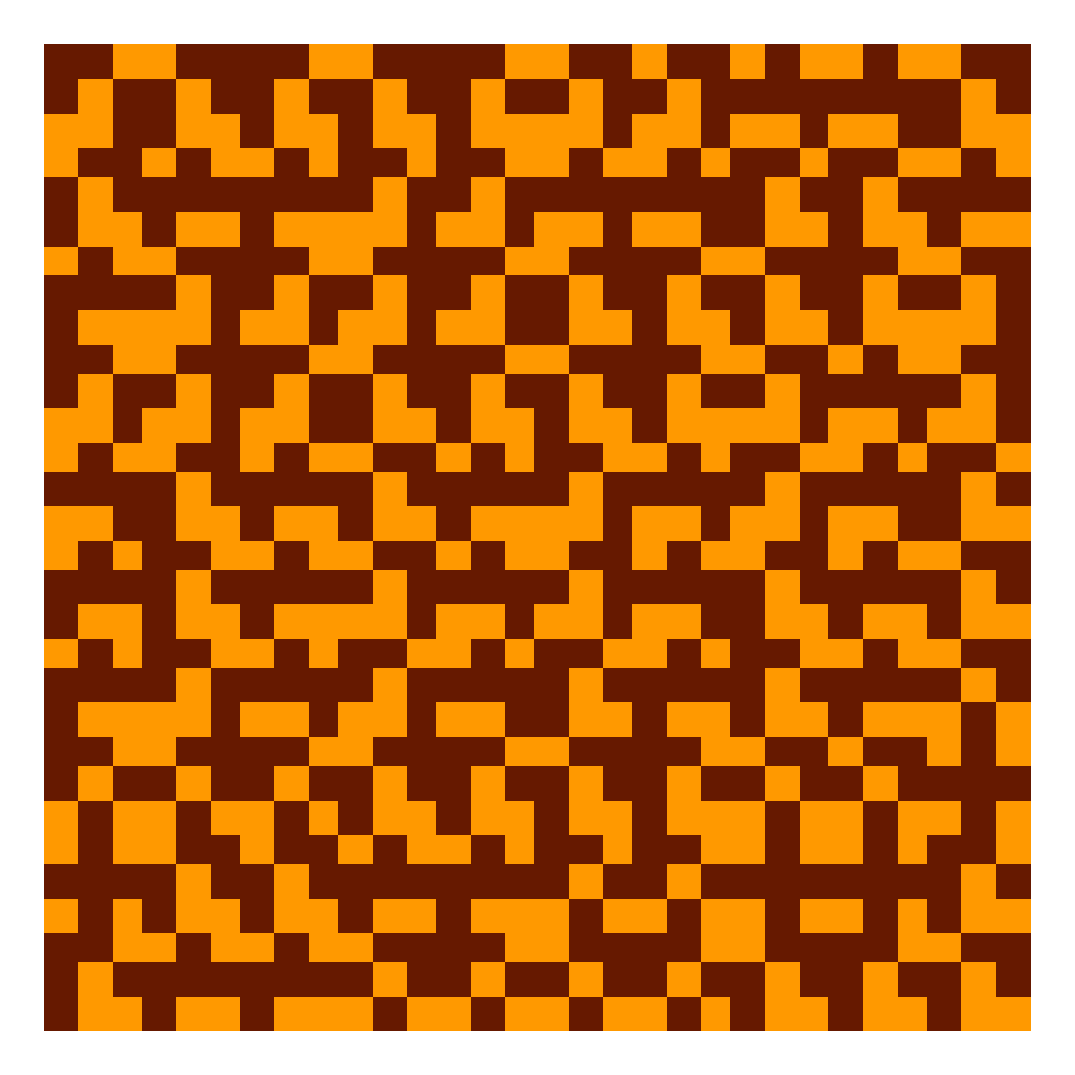
\includegraphics[width=6.2cm]{2005-ae-raster-pe}
&
 \includegraphics[width=6.2cm]{2005-ae-raster-diag}
\\
(a)&(b)&(c) \\
$\;$\\
 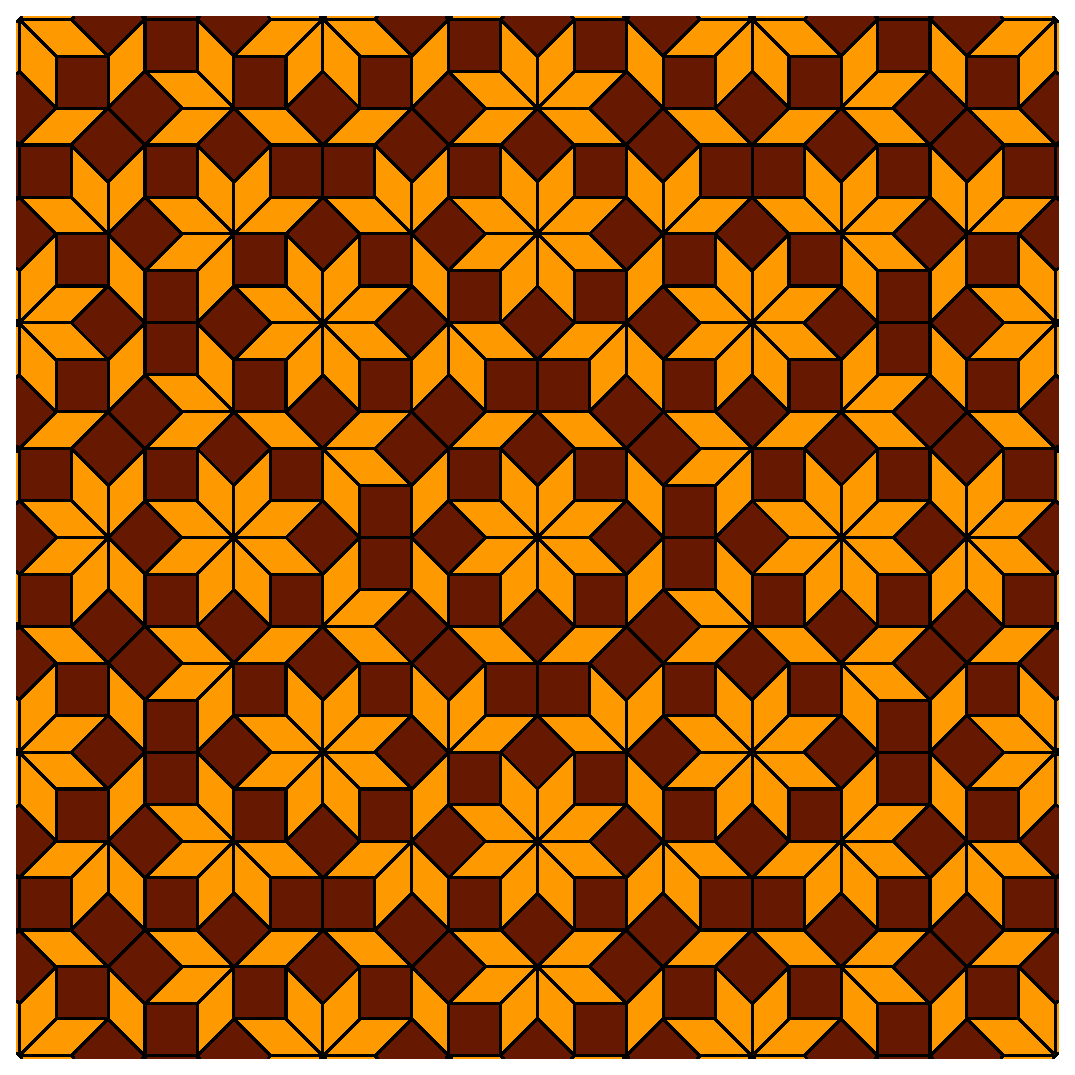
\includegraphics[width=5.87cm]{2005-ae-tiling}
&
 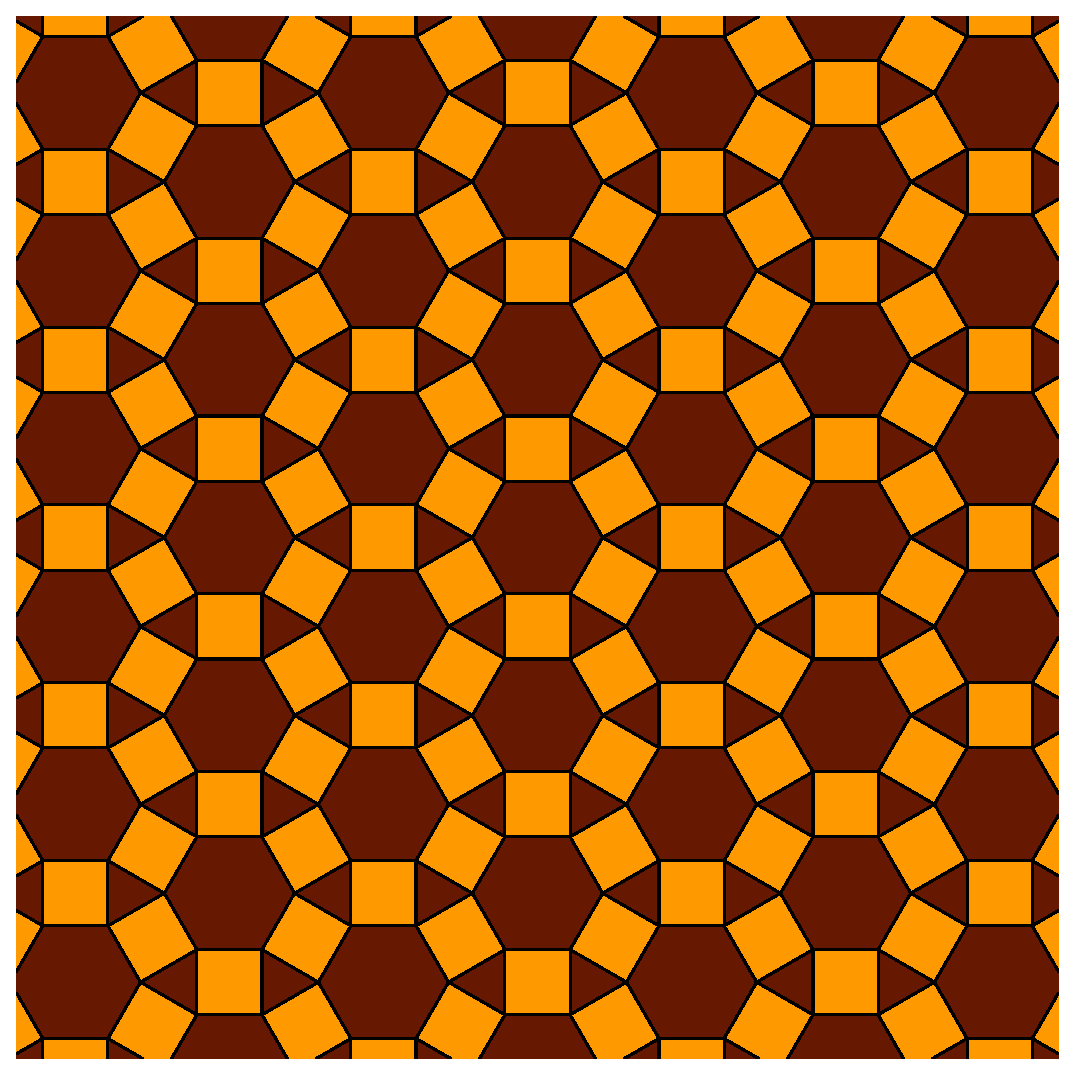
\includegraphics[width=5.87cm]{2005-ae-tess}
&
 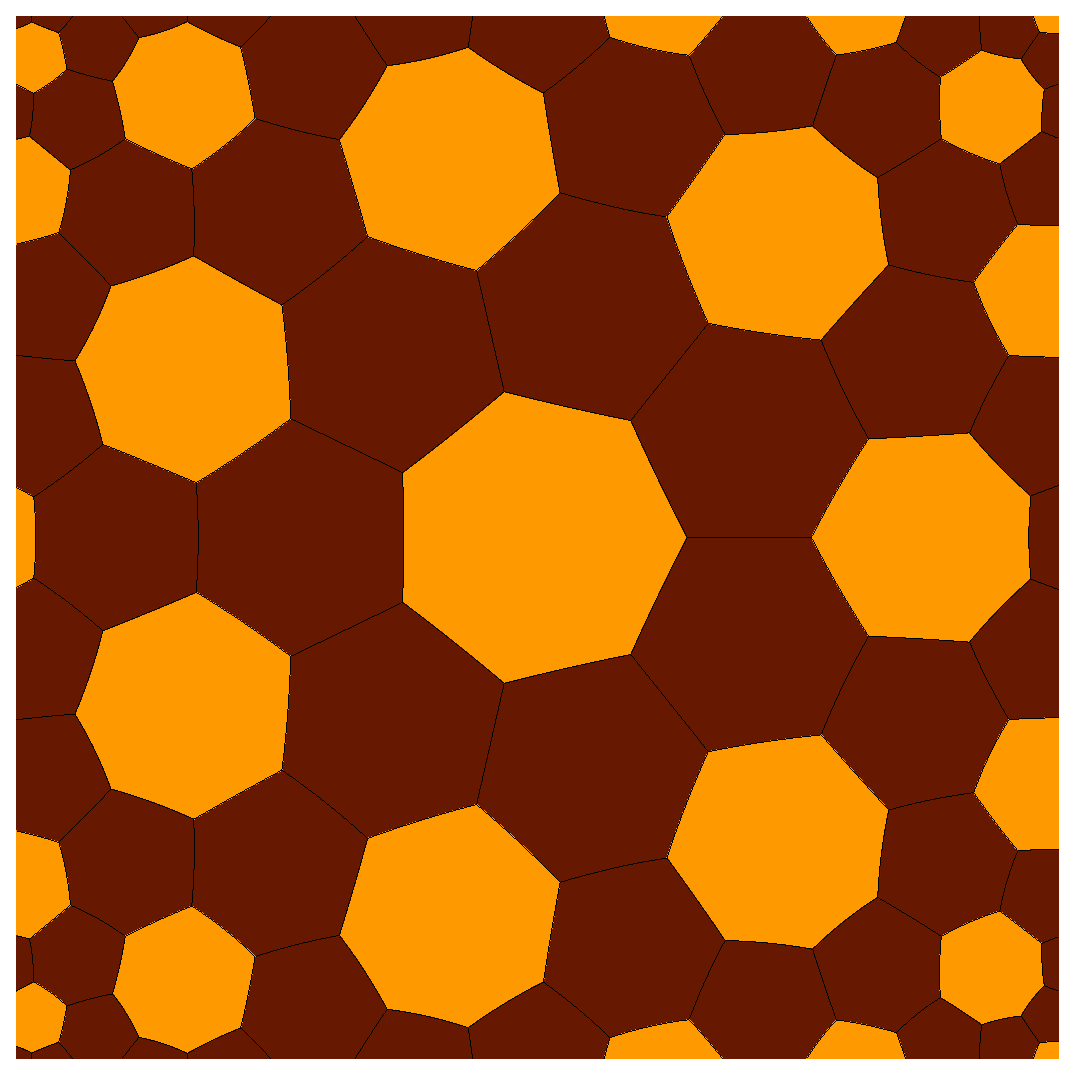
\includegraphics[width=5.87cm]{2005-ae-tess2}
\\
(d)&(e)&(f)\\
$\;$\\
 \includegraphics[width=5.87cm]{2005-ae-tess3}
&
 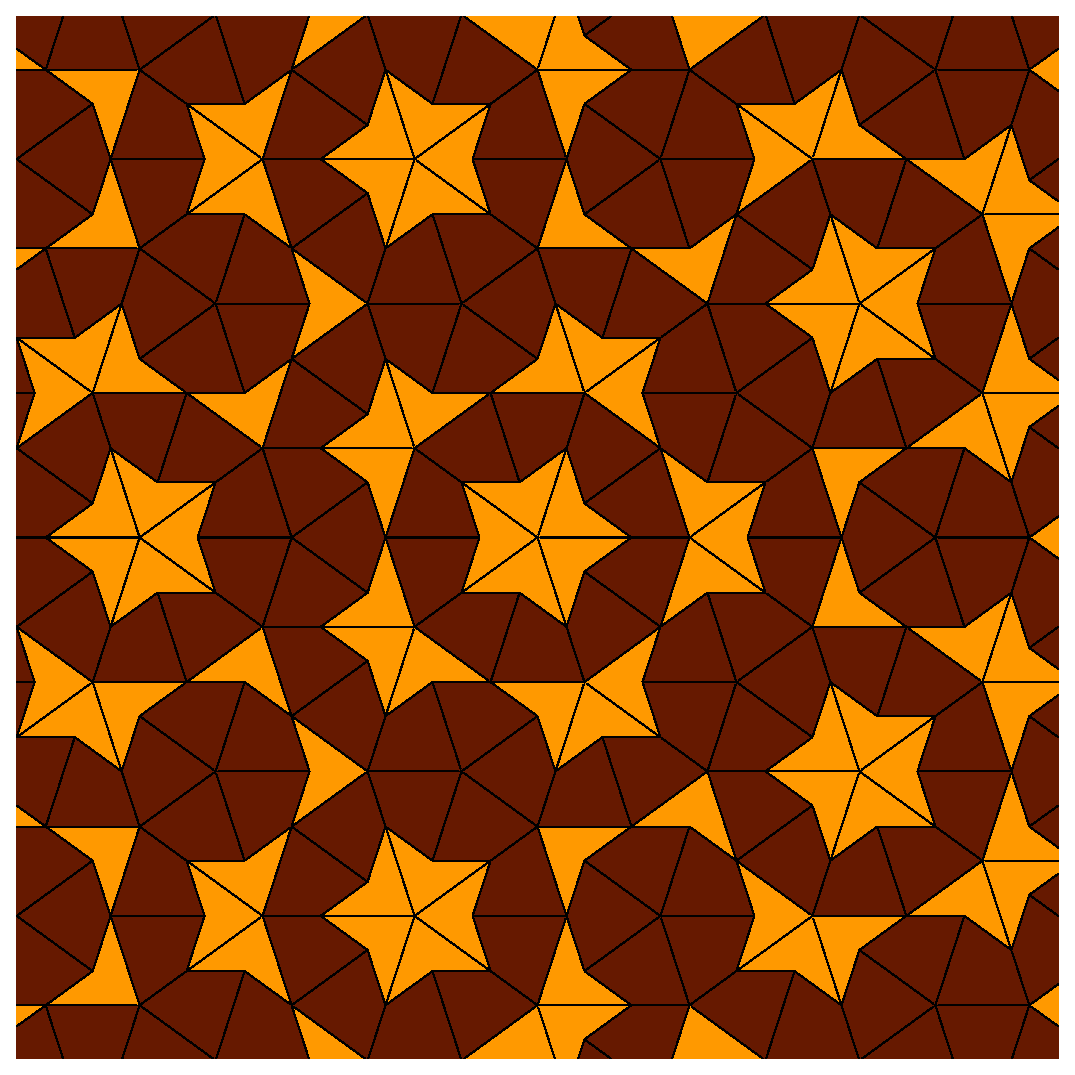
\includegraphics[width=5.87cm]{2005-ae-penrose}
&
 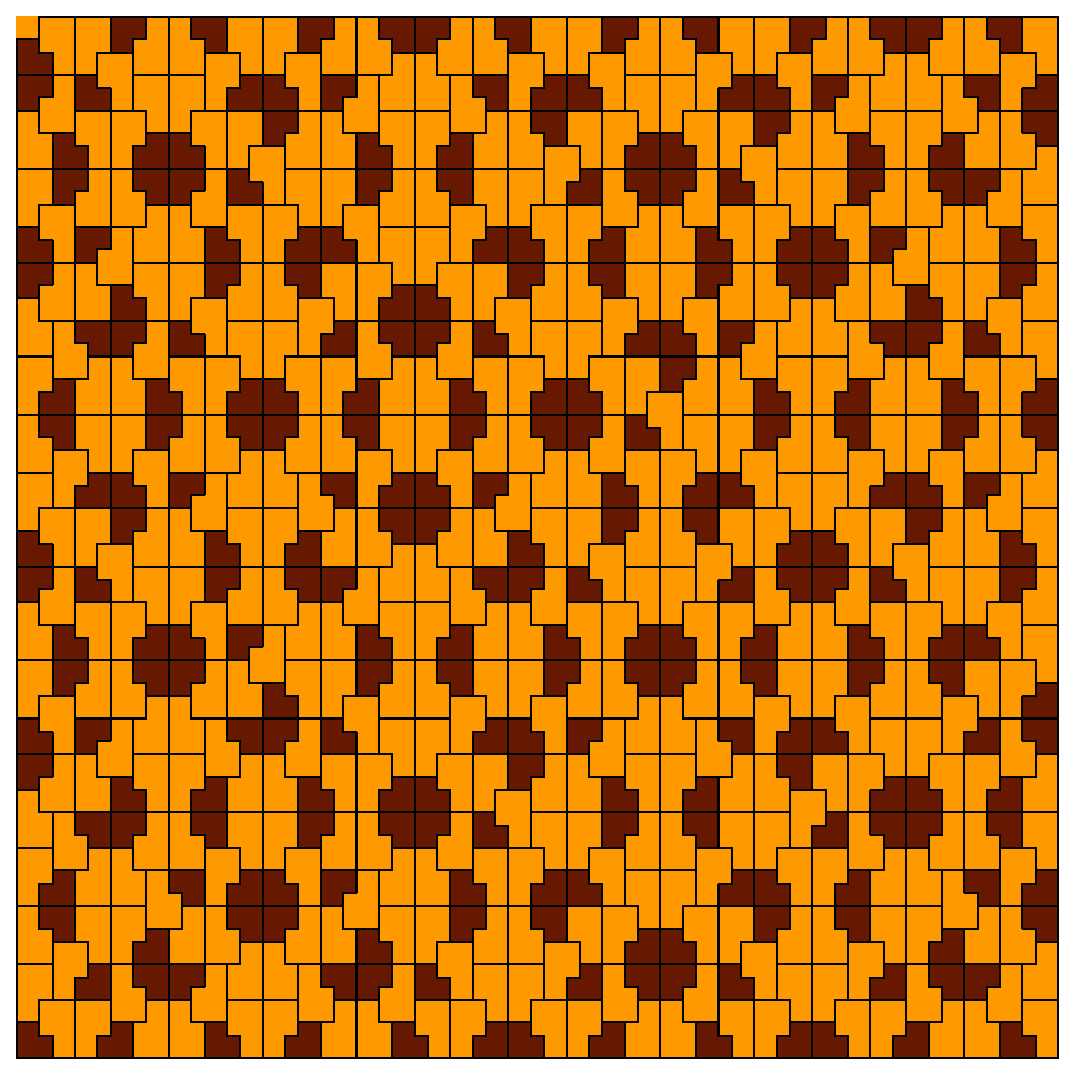
\includegraphics[width=5.87cm]{2005-ae-ammann}
\\
(g)&(h)&(i)\\
\end{tabular}
\end{center}
   \caption{Raster graphics
(a) from white noise;
(b) from permutations in a quantum \cite{DonSvo01}
and automaton \cite{svozil-2004-kyoto,svozil-2003-garda} state discrimination problem;
(c) from regular tessellation through repetition;
(d) Tiling obtained from the projection of a dimensional hypercube with
an algorithm by  Grimm and Schreiber  \cite{grimm-schr-02};
(e-g) Tilings from
an algorithm by  Sremcevic and Sazdanovic (MathSource 4540);
%http://library.wolfram.com/infocenter/MathSource/4540/
(h) Tiling from
an algorithm by Lyman P. Hurd (MathSource 595);
%http://library.wolfram.com/infocenter/MathSource/595/
(i) Ammann aperiodic tiling from
an algorithm by Sasho Kalajdzievski (MathSource 4273);
%http://library.wolfram.com/infocenter/MathSource/4273/
}
   \label{2005-ae-raster-wn}
 \end{figure}

\subsection{Morphing and crossing of existing forms}

This variation has been borrowed from Genetic Algorithms \cite{goldberg:89,holland:92a,mitchell}.
It is
the deliberate use of natural forms such as leaves, trees, waves and so on,
morphing, crossing and blending them into existing functional and structural
entities. The shape of Ionic and Corinthian Capitals,
as depicted in Fig.~\ref{2005-ae-owen}(c), are such examples. Imagine a Greek or Roman temple such as the
Erechtheum in Athens build in plain Bauhaus or International Style!

%http://www.perseus.tufts.edu/cgi-bin/imbrow
\begin{figure}
\begin{center}
\begin{tabular}{c}
 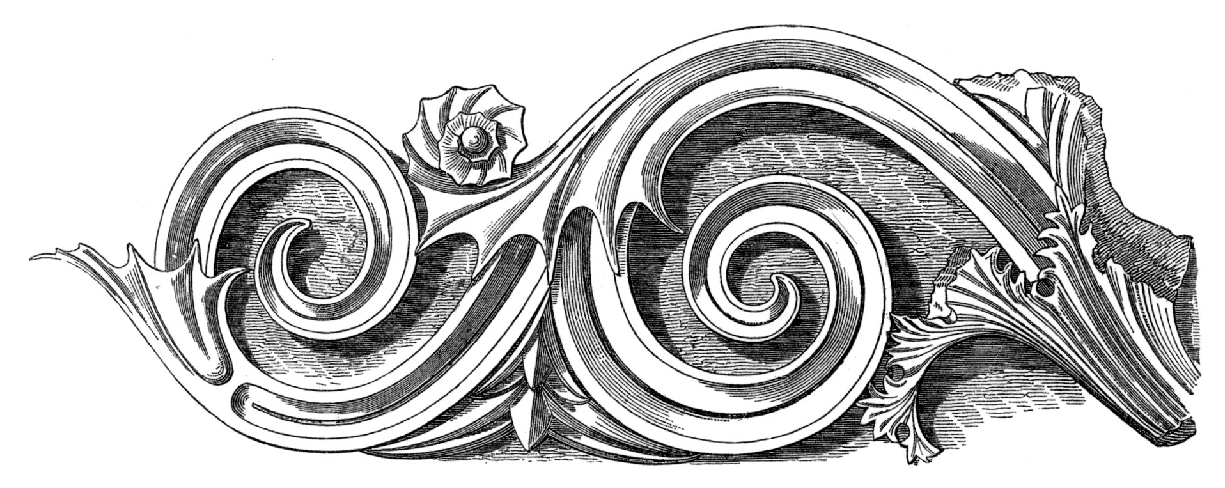
\includegraphics[width=10cm]{2005-ae-greekornament1}\\
(a)\\
$\;$\\
 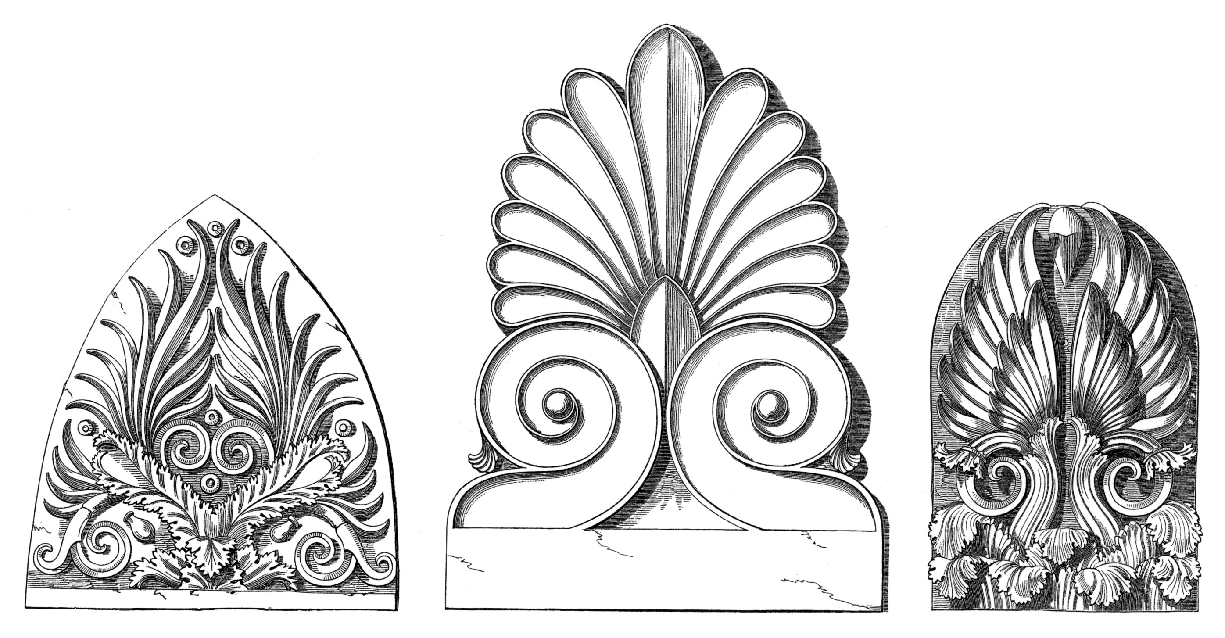
\includegraphics[width=11cm]{2005-ae-greekornament2}\\
(b)\\
$\;$\\
 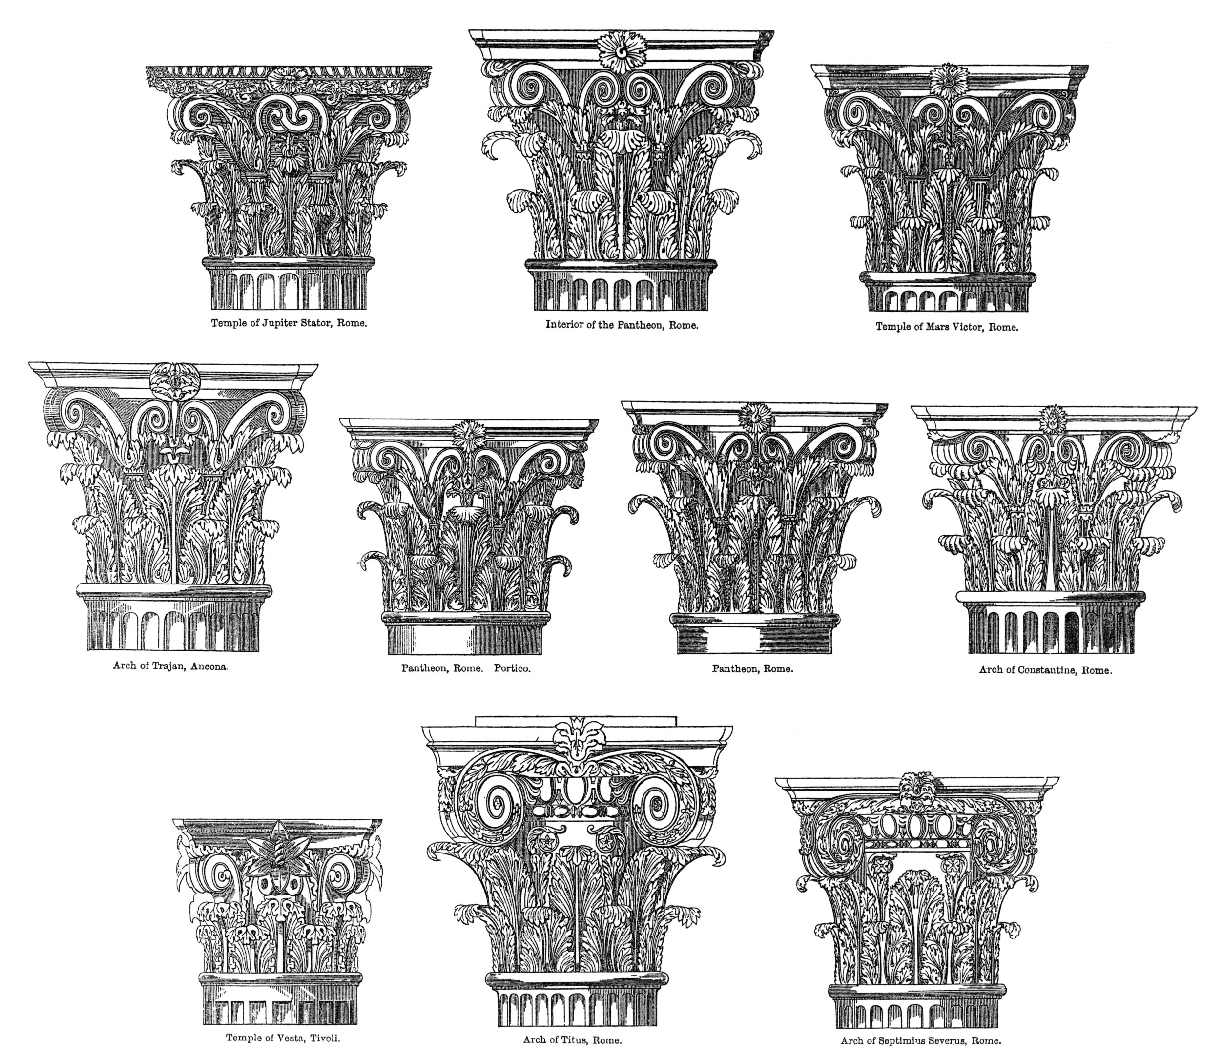
\includegraphics[width=13cm]{2005-ae-romanornament1}\\
(c)
\end{tabular}
\end{center}
   \caption{(a) Greek ornament from the Chorage Monument of Lysicrates, Athens; by Lewis Vulliamy and
reprinted by Owen Jones \cite{jones-goo};
(b) Greek ornament from left to right: upper part of a stele,
termination of the marble tiles of the Pantheon;
the upper part of a stele;
by Lewis Vulliamy and
reprinted by Owen Jones \cite{jones-goo};
(c) Roman Corinthian and Composite Capitals reduced from Taylor and Cresy's {\it Rome} \cite{Tay-Cr} and
reprinted by Owen Jones \cite{jones-goo};
%Racinet's Historic Ornament in Full Color (Dover Pictorial Archive) (Paperback)
}
   \label{2005-ae-owen}
 \end{figure}


\subsection{Permutation}

Permutations are a means to repeat one and the same formal message over and
over again without repeating it syntactically. Strictly speaking, it should
be considered in the symmetry section below. One of the decisive features of
permutations are the reversibility, the ``one-to-one-ness'' of the
associated transformations.
Fig.~\ref{2005-ae-raster-wn}(b) depicts a permutation pattern previously generated
in the context of quantum state discrimination
\cite{DonSvo01,svozil-2002-statepart-prl,svozil-2004-kyoto,svozil-2003-garda}.

\subsection{Self-similarity}

Self-similar ``fractal''
\cite{mandelbrot-77,mandelbrot-83,falconer1,falconer2}
structures
have been discussed intensively
in the context of the creation authentically looking landscapes
\cite{voss85}
and architectural form
\cite{bovill,jencks}, as well as music \cite{gard-78} and paintings \cite{taylor-99}.
As demonstrated by the image compression techniques
from iterated functions systems
\cite{barnsley:88},
fractals are generated by
the successive iteration of certain non-linear mappings.

It should be realised however, that although fractal forms abound in nature,
their virtually generated doubles often tend to appear boring and
artificial. A combination of fractal symmetry and random mutation may be a
good recipe for creating interesting patterns.


\subsection{Repetition}

Repetition of patterns and reproduction of natural forms
such as the ones in Fig.~\ref{2005-ae-raster-wn}(c,e,g) may be a great
design resource.
It should be noted that without any modifications
such as mutation, the repetition of small structures can be decoded very easily
and thus may appear monotonous. One should, however, not underestimate
the joy people experience by listening to something they already know
\cite{feynman-law}!



\subsection{Symmetry}

Ornamentation by symmetric patterns is an ancient method.
Contemporary mathematics offers a pandemonium of different symmetric patterns
\cite{gruenbaum-tiling},
the formally most advanced being aperiodic tilings
\cite{baake-02,grimm-schr-02}.
Figs.~\ref{2005-ae-raster-wn}(d,f,h,i) depict such aperiodic floor tilings.
These tilings would not have been possible a few years ago
and therefore are not realized in any historic building.



%\begin{figure}
%%\centerline{\reserve{19.0cm}{24.5cm}{pdf: image width 19.0cm (2005-Jupiter.jpg)}}
%   \caption{Jupiter
%(\copyright NASA)}
%   \label{2005-Jupiter}
% \end{figure}


%\begin{figure}
%%\centerline{\reserve{19.0cm}{24.5cm}{pdf: image width 19.0cm (2005-ae-East_Mediterranean_MER_RR_Date_20040721_Time_081824_Orbit_12500.jpg)}}
%  \caption{East-Mediterranean - MERIS - 21 July 2004
%(\copyright ESA/MERIS)}
%   \label{2005-ae-East_Mediterranean_MER_RR_Date_20040721_Time_081824_Orbit_12500}
% \end{figure}

\section{Human art versus computer generated design versus nature-beauty}

So far nothing has been said about human originality and artistic talent.
Indeed, the more one attempts to argue for the necessity and feasibility of
automated creation of ornamentation in accord with nature-beauty, the more
it becomes clear how brilliant, gratifying and truly enjoyable human
artistic expressions can be.

Consider, for example, the traditional ornaments collected by Owen Jones
\cite{jones-goo} and depicted in Fig.~\ref{2005-ae-owen}, the stucco created by Santino Bussi and
depicted in Fig.~\ref{2005-ae-bospiral}, and Jan Van Huysum's bouquet of flowers
in Fig.~\ref{2005-ae-JanVanHuysum_Blumenstrauss}.
From
these experiences it may appear even questionable whether the automation of
pattern formation will ever be capable to fully substitute or outperform
human art. One is reminded of similar debates in artificial intelligence
research and the controversy between semantics and the associated syntax,
which has so vividly been expressed in Searle's ``Chinese room'' metaphor
\cite{searl-80a,searl-84} against strong artificial intelligence;
or Weizenbaums artificial communicator ``Eliza.''
\begin{figure}
\centerline{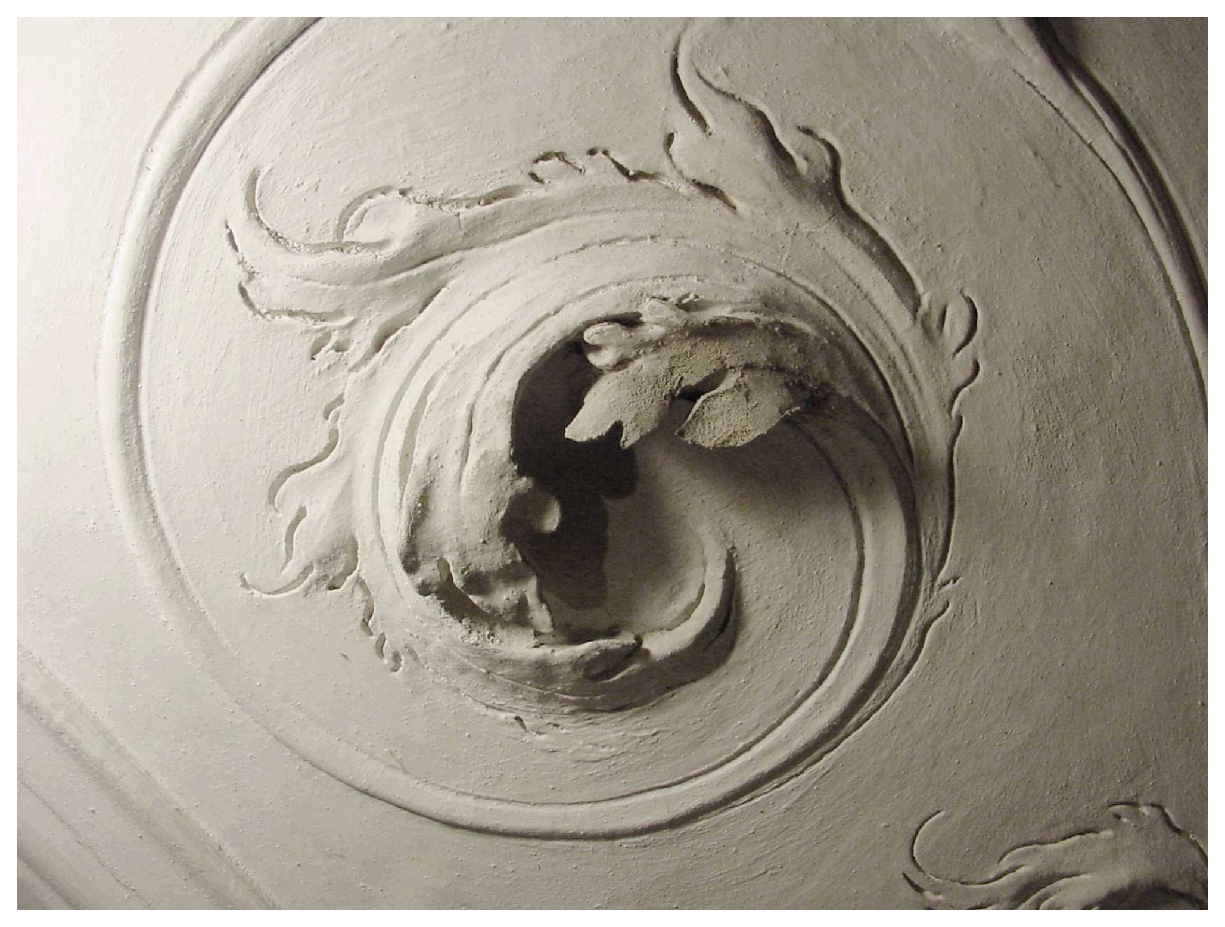
\includegraphics[width=19cm]{2005-ae-bospiral}}
   \caption{Santino Bussi (1664-1736) Stucco detail in the Sala Terrena of the Garden Palais
 Liechtenstein, after 1700, Vienna, Austria
(\copyright Sammlungen des F\"ursten von und zu Liechtenstein, Vaduz.
URL http://www.liechtensteinmuseum.at)}
   \label{2005-ae-bospiral}
 \end{figure}
\begin{figure}
\centerline{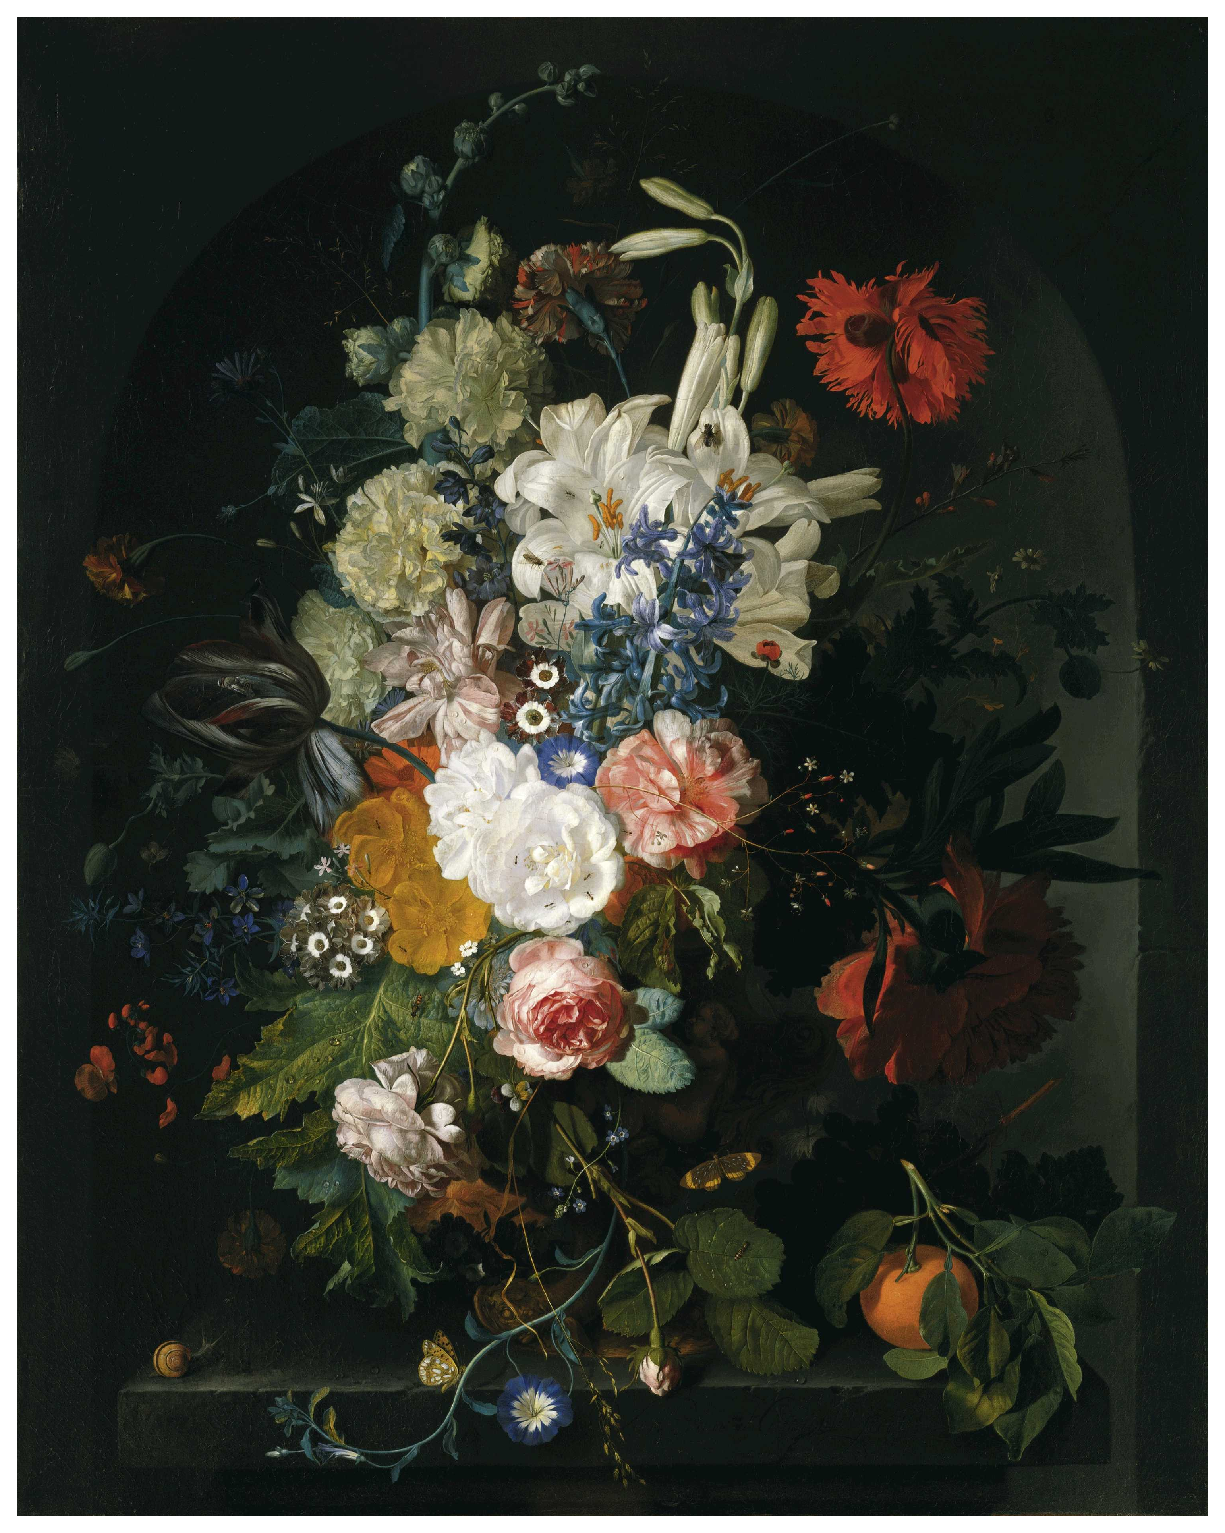
\includegraphics[width=19cm]{2005-ae-JanVanHuysum_Blumenstrauss}}
   \caption{Jan Van Huysum, Flowers
(\copyright Sammlungen des F\"ursten von und zu Liechtenstein, Vaduz.
URL http://www.liechtensteinmuseum.at)}
   \label{2005-ae-JanVanHuysum_Blumenstrauss}
 \end{figure}

In view of the preliminary nature of these issues, let me just ask a few
questions: Is ``algorithmic art'' \cite{stiny} not a \textit{contradictio in adjecto,} an inconsistency in the adjective
modifying a noun, as in ``round square?'' Why do modern biology books still
use drawings made by humans rather than photography? Is nature-beauty just
the expression of deeper forms which are only revealed by human artistic
talent? Is the human mind capable of condensing the ``essence'' of natural
form? That is, are natural forms mere shadows of hidden objects as in
Plato's cave metaphor---and are artists capable of recognising the ``real''
objects behind those shadows?---Maya covering an illusory world of the senses?
What is it that makes Reality feel ``so real? '' The song of a nightingale
is beautiful, but is Korngold's ``Violanta,'' Bach's
``Matth\"{a}uspassion,'' or Mahler's ``Sixth Symphony'', his ``Song of the
Earth,'' Sch\"onberg's ``Gurrelieder,''
Schreker's ``Irrelohe,'' or Wagner's ``Tristan und Isolde'' even more so? How is it possible
for those masters to distil and create beauty from their experiences? May
this be indication for transcendence and dualism?



\section{Summary and outlook}

We have argued for the necessity of ornamentation, decoration and the
presence of nature-beauty as a precondition for aesthetic acceptance. We
have discussed bounds from above and from below on artistic expression: art
can neither exist in a scheme dominated by chaos, randomness, arbitrariness and
white noise, nor can it exist in a regime dominated by too much order, monotony and
dullness. Thereby, we have in mind statistical and algorithmic measures and
methods to evaluate and automatically generate ornamental forms.

For those desperate for beauty and surrounded by ugliness,
let me add a quite simple advise: look
upward to the sky and watch the clouds pass by;
go to the woods; take a pilgrimage, go walkabout!
No despot so far in human history was able to eliminate clouds, plants,
the sunrise and sunset.

Another practical suggestion is the construction of a network of ``green corridors''
through city centers. These corridors should be covered with lush vegetation
and should allow pedestrians and probably also cyclists to traverse
passages of ugly facades and constructions, which would be effectively coated
by natural ornamentation.
Another possibility would be to systematically cover great parts of city facades by plants.


Creating enjoyable habitats for the human mind by algorithmic methods
presents a great challenge. Therefore, it is promising and gratifying to
look into the future of virtual reality modelling by also looking back at
the traditions of form, decoration and ornament. So much beauty is awaiting
us in those universes when we have shaken off the armour of hatred for the
forms which we always loved and sought. By wisely maintaining our cultural
as well as our human heritage in evenly suspended attention (to borrow the
wording ``gleichschwebende Aufmerksamkeit'' from Freudian psychoanalysis),
it will be a liberation from a certain kind of totalitarian modernity which,
whenever dominant, has created deserts of monotony and ugliness, and a step
forward to enjoy ourselves within the universes which await us in the years
to come.

\section*{Acknowledments}
I would like to express my special thanks to Ross Rhodes
for critically reading and revising the manuscript.
Thanks go also to (in lexicographic order)
Tim Bo,
Georg Franck-Oberaspach,
G\"unter Krenn,
Christian Schreibm\"uller,
and
Udo Wid
for discussions and references.
Many ideas grew from a research cooperation with Klaus Ehrenberger
of the Medical University of Vienna on the coding and processing of
stimuli by cochlear implants, a direct artificial interface to the cortex.
Almost needless to say,
I take full responsibility for controversial statements.
Reproductions of Figs.~\ref{2005-ae-flooring}, \ref{2005-ae-bospiral}, and \ref{2005-ae-JanVanHuysum_Blumenstrauss}
with kind permission of the Sammlungen des F\"ursten von und zu Liechtenstein.

\bibliography{svozil}
\bibliographystyle{osa}

\end{document}


\begin{figure}
%\centerline{\reserve{12.0cm}{10.0cm}{pdf: image width 12.0cm (2005-ae-klimt-facade_LW40.jpg)}}
   \caption{Facade of apartment house Linke Wienzeile 40 (Majolikahaus, 1898 - 1899), Otto Wagner, architect, tilings by Gustav Klimt. Loos called this ``tattood arcitecture.''
(\copyright Karl Svozil)}
   \label{2005-ae-klimt-facade_LW40}
 \end{figure}


\begin{figure}
%\centerline{\reserve{19.0cm}{15.0cm}{pdf: image width 19.0cm (2005-ae-raspberries.jpg)}}
   \caption{Rasperries from Rust, Lower Austria, July 9, 2000
(\copyright Karl Svozil)}
   \label{2005-ae-raspberries}
 \end{figure}



<< DiscreteMath`

(*** PERMUTATIONS***)

p9 = Permutations[{1, 2, 3, 4, 5, 6, 7, 8, 9}];

trits[x1_, x2_, x3_, x4_, x5_, x6_, x7_, x8_, x9_] := {Sort[{x1, x2, x3}],
      Sort[{x4, x5, x6}], Sort[{x7, x8, x9}], Sort[{x1, x4, x7}],
      Sort[{x2, x5, x8}], Sort[{x3, x6, x9}]};

part3 = Union[
      Table[trits[p9[[i, 1]], p9[[i, 2]], p9[[i, 3]], p9[[i, 4]], p9[[i, 5]],
          p9[[i, 6]], p9[[i, 7]], p9[[i, 8]], p9[[i, 9]]], {i, 9!}]];

Length[part3]

color1 = {{1, 0.6, 0}, {0.4, 0.1, 0}};
a1 = 0.5; a2 = 0.5; b1 = 0.5; b2 = 0.1; c1 = 0; c2 = 0;
garr = Table[color = Table[{0, 0, 0}, {iii, 1, 9}];
      color[[part3[[i, 1, 1]], 1]] += a1;
      color[[part3[[i, 1, 2]], 1]] += a1;
      color[[part3[[i, 1, 3]], 1]] += a1;
      color[[part3[[i, 4, 1]], 1]] += a2;
      color[[part3[[i, 4, 2]], 1]] += a2;
      color[[part3[[i, 4, 3]], 1]] += a2;
      color[[part3[[i, 2, 1]], 2]] += b1;
      color[[part3[[i, 2, 2]], 2]] += b1;
      color[[part3[[i, 2, 3]], 2]] += b1;
      color[[part3[[i, 5, 1]], 2]] += b2;
      color[[part3[[i, 5, 2]], 2]] += b2;
      color[[part3[[i, 5, 3]], 2]] += b2;
      color[[part3[[i, 3, 1]], 3]] += c1;
      color[[part3[[i, 3, 2]], 3]] += c1;
      color[[part3[[i, 3, 3]], 3]] += c1;
      color[[part3[[i, 6, 1]], 3]] += c2;
      color[[part3[[i, 6, 2]], 3]] += c2;
      color[[part3[[i, 6, 3]], 3]] += c2;
      colarray = Partition[Table[

            If [color[[ii, 1]] + color[[ii, 2]] + color[[ii, 3]] >= 0.6,
              RGBColor[1, 0.6, 0], RGBColor[0.4, 0.1, 0] ], {ii, 1, 9}], 3];
      Graphics[RasterArray[colarray], AspectRatio -> 1, Frame -> False], {i, 3100, 3200}];
Show[GraphicsArray[Partition[garr, 10], GraphicsSpacing -> -0.1]]

Export["c:/mytex/2005-ae-raster-pe.eps", %, "EPS", ImageSize -> 500]


(*** RANDOMIZATION ***)

color = {{1, 0.6, 0}, {0.4, 0.1, 0}};
colarray =
    Table[Apply[RGBColor, color[[Random[Integer] + 1]]], {ii, 1, 1600}];

Show[Graphics[RasterArray[Partition[colarray, 40]], AspectRatio -> 1,
    Frame -> False]]



Export["c:/mytex/2005-ae-random.eps", %, "EPS", ImageSize -> 500]


(***********  regular ************)

color={{1,0.6,0},{0.4,0.1,0}};
colarray=Table[Apply[RGBColor,color[[  Mod[ii+1,2]+1  ]] ],{ii,1,400}];

Show[Graphics[RasterArray[Partition[colarray,21]],AspectRatio\[Rule]1,
    Frame\[Rule]False]]

Export["c:/mytex/2005-ae-raster-diag.eps", %, "EPS", ImageSize -> 500]


% http://library.wolfram.com/infocenter/BySubject/Mathematics/Geometry/Tiling/

(*************** TILINGS *******************)

Show[PlotOctagonalTiling[til2, 3/1000, 0, False, False, False,
      False, {0, 0, 0}, 1, {1, 0.6, 0}, {0.4, 0.1, 0}, {1, 0, 0}, {1, 0, 1}]];

Show[PlotOctagonalTiling[CutOctagonalPatch[til3, {0, 0}, 2000], 5/1000, 0,
      False, False, False, False, {0, 0, 0},
      0, {1, 0.6, 0}, {0.4, 0.1, 0}, {1, 0, 0}, {1, 0, 1}]];

Show[PlotOctagonalTiling[til2, 2/1000, 0, False, False, False,
      False, {0, 0, 0}, 0, {1, 0.6, 0}, {0.4, 0.1, 0}, {1, 0, 0}, {1, 0, 1}]];

Export["c:/mytex/2005-ae-tiling.eps", %, "EPS", ImageSize -> 500]


 AspectRatio -> 1.2,
                PlotRange -> {{-16,16},{-4.8*4,4.8*4}}]];
<< C:/MYTEX/tilings/GridMethod.m
PlotDualTiling[DualizeGrid[7, -6, 6], True, False, 1/400];

Export["c:/mytex/2005-ae-tiling2.eps", %, "EPS", ImageSize -> 500]



TessShow[{4, 3, 4, 6}, NPolygons -> 1000,
  PolygonColor -> {1 -> RGBColor[1, 0.6, 0], 3 -> RGBColor[0.4, 0.1, 0],
      2 -> RGBColor[0.4, 0.1, 0]}, Thickness -> 0.002,
  PlotRange -> {{-8, 8}, {-8, 8}}]
Export["c:/mytex/2005-ae-tess.eps", %, "EPS", ImageSize -> 500]


c1 = TessGraphics[{6, 6, 7}, NPolygons -> 500, Annotate -> Off,
      Thickness -> 0.0005,
      PolygonColor -> {6 -> RGBColor[0.4, 0.1, 0], 7 -> RGBColor[1, 0.6, 0]}];
Show[c1, PlotRange -> {{-0.65, 0.65}, {-0.65, 0.65}}];
Export["c:/mytex/2005-ae-tess2.eps", %, "EPS", ImageSize -> 500]


TessShow[{3, 3, 4, 3, 4}, PlotRange -> {{-4, 4}, {-4, 4}}, NPolygons -> 200,
  PolygonColor -> {1 -> RGBColor[1, 0.6, 0], 3 -> RGBColor[0.4, 0.1, 0],
      2 -> RGBColor[0.2, 0.1, 0]}, Thickness -> 0.002]

Export["c:/mytex/2005-ae-tess3.eps", %, "EPS", ImageSize -> 500]


<< C:/MYTEX/tilings/Penrose.m
ColorGraph[Deflate[Sun, 5]]
Export["c:/mytex/2005-ae-penrose.eps", %, "EPS", ImageSize -> 500]

<< C:/MYTEX/tilings/AmmannTiling.m
Show[colorGraphA3[deflate[la3Tile, 14], la3Color -> RGBColor[1, 0.6, 0],
    sa3Color -> RGBColor[0.4, 0.1, 0]], DisplayFunction -> $DisplayFunction,
  AspectRatio -> 1]
Export["c:/mytex/2005-ae-ammann.eps", %, "EPS", ImageSize -> 500]

